%Dokumentinformationen
\newcommand{\titleinfo}{Informatik - Zusammenfassung}
\newcommand{\authorinfo}{C.Renda, R. von Reding}
\newcommand{\versioninfo}{$Revision: $ \today}

%Weitere Autoren %%%%%%%%%%%%%%%%%%%%%%%%%%%%%%%%%%%%%%%%%%%%%%%%%%%%%%%%%%%%%%%%%%%%%%
%C.Renda

% standard header
%Schriftgr�sse, Layout, Papierformat, Art des Dokumentes
\documentclass[8pt,twoside,a4paper,fleqn]{extarticle}
\usepackage{extsizes}
%Einstellungen der Seitenraender
\usepackage[left=0.5cm,right=0.5cm,top=0.5cm,bottom=0.5cm,includeheadfoot,landscape=true]{geometry}
% Sprache, Zeichensatz, packages
%\usepackage[latin1]{inputenc}
\usepackage[english,ngerman]{babel}
\usepackage[utf8]{inputenc}
\usepackage{cancel}

%\usepackage[ngerman]{babel,varioref}
\usepackage{amssymb,amsmath,fancybox,graphicx,color,lastpage,wrapfig,fancyhdr,hyperref,verbatim}
\usepackage[T1]{fontenc}

\newcommand{\licence}{CC BY-NC-SA}

%pdf info
\hypersetup{pdfauthor={\authorinfo},pdftitle={\titleinfo},colorlinks=false}
%linkbordercolor=white
\author{\authorinfo}
\title{\titleinfo}

%Kopf- und Fusszeile
\pagestyle{fancy}
\fancyhf{}
%Linien oben und unten
\renewcommand{\headrulewidth}{0.5pt} 
%\renewcommand{\footrulewidth}{0.5pt}

\fancyhead[L]{\titleinfo{ }\tiny{(\versioninfo)}}
%Kopfzeile rechts bzw. aussen
\fancyhead[R]{Seite \thepage { }von \pageref{LastPage}}

%Fusszeile
%\fancyfoot[L]{\footnotesize{\authorinfo}}
%\fancyfoot[R]{\footnotesize{\today}}
%\fancyfoot[C]{\footnotesize{\licence \quad $\rightarrow$ \href{https://github.com/HSR-Stud}{Github: HSR-Stud}}}

%Programmausschnitte

\usepackage{listings}
%\usepackage{lstlinebgrd}

\definecolor{bgGray}{rgb}{0.95,0.95,0.95}
\definecolor{stringColor}{rgb}{0.16,0.00,1.00}
\definecolor{annotationColor}{rgb}{0.39,0.39,0.39}
\definecolor{keywordColor}{rgb}{0.50,0.00,0.33}
\definecolor{commentColor}{rgb}{0.25,0.50,0.37}

\lstdefinestyle{cpp}{ 
	%linebackgroundcolor={\ifodd\value{lstnumber}\color{bgGray}\else\color{white}\fi},   % choose the background color; you must add \usepackage{color} or \usepackage{xcolor}; should come as last argument
	backgroundcolor=\color{bgGray},
	basicstyle=\normalsize\ttfamily,        % the size of the fonts that are used for the code
	breakatwhitespace=false,         % sets if automatic breaks should only happen at whitespace
	breaklines=true,                 % sets automatic line breaking
	captionpos=none,                    % sets the caption-position to bottom
	commentstyle=\color{commentColor},    % comment style
	deletekeywords={...},            % if you want to delete keywords from the given language
	escapeinside={\%*}{*)},          % if you want to add LaTeX within your code
	extendedchars=true,              % lets you use non-ASCII characters; for 8-bits encodings only, does not work with UTF-8
	frame=tb,	                  	 % adds a frame around the code
	keepspaces=true,                 % keeps spaces in text, useful for keeping indentation of code (possibly needs columns=flexible)
	keywordstyle=\color{keywordColor}\bfseries,   % keyword style
	language=C++,                    % the language of the code
	morekeywords={*,...},            % if you want to add more keywords to the set
	numbers=none,                    % where to put the line-numbers; possible values are (none, left, right)
	numbersep=3pt,                   % how far the line-numbers are from the code
	numberstyle=\footnotesize\color{codeGray}, % the style that is used for the line-numbers
	rulecolor=\color{black},         % if not set, the frame-color may be changed on line-breaks within not-black text (e.g. comments (green here))
	showspaces=false,                % show spaces everywhere adding particular underscores; it overrides 'showstringspaces'
	showstringspaces=false,          % underline spaces within strings only
	showtabs=false,                  % show tabs within strings adding particular underscores
	stringstyle=\color{stringColor},     % string literal style
	tabsize=2,	                   % sets default tabsize to 2 spaces
	title=\lstname                   % show the filename of files included with \lstinputlisting; also try caption instead of title
}


 % ./header.tex nicht editieren (Projekt LaTeX-Header benutzen)

%%%%%%%%%%%%%%%%%%%%%%%%%%%%%%%%%%%%%%%%%%%%%%%%%%%%%%%%%%%%%%%%%%%%%%%%%%%%%%%%%%%%%%%%%%%%%%%%
% Neue Befehle und Definitionen                
%%%%%%%%%%%%%%%%%%%%%%%%%%%%%%%%%%%%%%%%%%%%%%%%%%%%%%%%%%%%%%%%%%%%%%%%%%%%%%%%%%%%%%%%%%%%%%%
% This is needed for one more subsection, ex. 1.1.1.1, is called by \paragraph{}
\usepackage{titlesec}
\setcounter{secnumdepth}{4}
\setcounter{tocdepth}{4}
\titleformat{\paragraph}
{\normalfont\normalsize\bfseries}{\theparagraph}{1em}{}
% Settings which are used to set the distance above and under the sections
%\titlespacing*{\paragraph}{0pt}{2.25ex plus 1ex minus .2ex}{1.0ex plus .2ex}
\titlespacing{\section}{0em}{0.5em}{0.5em}
\titlespacing{\subsection}{0em}{0.5em}{0.5em}
\titlespacing{\subsubsection}{0em}{0.5em}{0.5em}

% Linksbündig
\setlength\parindent{0ex}

% This is needed for a smaller itemlist, is called by \compactenum {}
\usepackage{paralist}

% This is needed for merging some columns in a table
\usepackage{multicol} 
\usepackage{multirow}

% This is needed for code listing
\usepackage[]{listings}
\lstset{literate=%
	{Ö}{{\"O}}1
	{Ä}{{\"A}}1
	{Ü}{{\"U}}1
	{ß}{{\ss}}1
	{ü}{{\"u}}1
	{ä}{{\"a}}1
	{ö}{{\"o}}1
	{~}{{\textasciitilde}}1
}

% This is needed to include Graphics
\usepackage{graphicx}

% This is needed for UML Diagrams
\usepackage{tikz}
\usepackage{pgf-umlcd}

% Courier font
\usepackage{courier}

\definecolor{red}{rgb}{1,0,0}
\definecolor{blue}{rgb}{0,0,1}
\definecolor{black}{rgb}{0,0,0}
\newcommand{\verweisc}[1]{$_{\textcolor{red}{\mbox{\small{C Kap. #1}}}}$}
\newcommand{\verweiscpp}[1]{$_{\textcolor{blue}{\mbox{\small{C++ Kap. #1}}}}$}
\newcommand{\verweisboth}[2]{$_{\textcolor{red}{\mbox{\small{C Kap. #1}}}}$$_{\textcolor{black}{\mbox{\small{, }}}}$$_{\textcolor{blue}{\mbox{\small{C++ Kap. #2}}}}$}
\newcommand{\verweishoch}[1]{${\textcolor{red}{\mbox{\small{Kapitel #1}}}}$}
\newcommand{\lc}[1]{\textit{\texttt{#1}}}

%Document Anfang
\begin{document}	


	\raggedbottom
	\lstset{style=cpp}
\begin{multicols*}{4}
	\section{Aufbau eines Programmes}

\begin{lstlisting}
#include <iostream> // Standart In-/ Output stream
#include <vector>		// Vector library
#include <cmath>		// Für math. funktionen	
#include <time.h>		// Zeitmessung
#include "headerfile.h" // Einbiden Headerfile
#define N 10	// defines jeglicher art

//structs, functions, enums

int main(void)
{
//programm code
return 0;
}
\end{lstlisting}


	\section{Variablen}

\begin{center}
	\begin{tabular}{ |l|l|l| } 
		\hline
		 \texttt{char} & 1 byte  8 bits. \\ 
		 \texttt{char16\_t} & At least 16 bits \\ 
		 \texttt{char32\_t} & At least 32 bits. \\ 
		\hline
		
		 \texttt{signed char} 			& Min 8 bits. \\ 
		 \texttt{signed short int} 	& Min 16 bits. \\ 
		 \texttt{signed int} 			& Min 16 bits. \\ 
		 \texttt{signed long int} 		& Min 32 bits. \\
		 \texttt{signed long long int} & Min 64 bits. \\
		\hline
		
 		
		 \texttt{unsigned char} 			& Min 8 bits. \\ 
		 \texttt{" short int} 		& Min 16 bits. \\ 
		 \texttt{"int} 			& Min 16 bits. \\ 
		 \texttt{" long int} 		& Min 32 bits. \\
		 \texttt{" long long int} 	& Min 64 bits. \\
		\hline
	\end{tabular}
\end{center}
\subsection{Variablennamen}
Keine Leerzeichen, Satzzeichen oder \_ Symbole Keine Zahl oder am Anfang case sensitivity – Gross - Kleinschreibung beachten

\subsection{Einfache Variablen deklarieren}
\begin{lstlisting}
int a,a2;   int b (1);
int b = 10;  int b {1};
float c = a*b - 0.5;
\end{lstlisting}
\subsection{Casts}
Änderung einer Variable in einen anderen Type
\begin{lstlisting}	
double a = 1.5; int b;
b = int (a);
b = (int) a; // b=1
7/2 = 3 , 7/(double)2 = 7/2.0 = 3.5
double(7/2) = 3.0 , int(19/10.0) = 1
\end{lstlisting}


\subsection{Enum}
Enum ist ein Aufzählungstyp. Die Konstanten aus der Enum
kann man im Programm verwenden.
\begin{lstlisting}	
enum farbe {ROT, BLAU, GELB};
farbe f = ROT;
if(f != BLAU) { }; 
\end{lstlisting}

\subsection{Hexadezimaler Code \& Adressen}
0,1,...,9,A,B,C,D,E,F (hex) anstelle von 0,1,...,14,15,16 (dec)
Adressen werden hexadezimal angegeben. $a,a+1,a+2,a+3,...$

\begin{center}
	\begin{tabular}{ ll } 
		\hline
int,float(4byte) & double (8byte)\\
\hline
0x22ff70 & 0x22ff70\\
0x22ff74 & 0x22ff78\\
0x22ff78 & 0x22ff80\\
		\hline
	\end{tabular}
\end{center}

\subsection{Fliesskommazahlen}
\begin{center}
	\begin{tabular}{ ll } 
		float&1b$\rightarrow$sign, 8b$\rightarrow$exp, 23b$\rightarrow$mantisse\\
		&Wert = $(-1)^{\texttt{S}} \cdot 2^{(\texttt{E-127})} \cdot (1.\texttt{F})$\\
		&Bsp: $0.125 = 2^{3} \Rightarrow \texttt{S} \rightarrow 0, \texttt{E} \rightarrow 124, \texttt{F} \rightarrow 0$\\
		\hline
		 & 0 | 01111100 | 00000000...0 = 0.125\\
		 & 0 | 01111111 | 00000000...0 = 1\\
		 & 1 | 01111111 | 11000000...0 = -1.75\\
		 & 0 | 00000000 | 00000000...0 = 0\\
		 & 0 | 11111111 | 00000000...0 = +infty\\
		 & 0 | 00000000 | 00000000...0 = NaN\\
		\hline
		double& 1b$\rightarrow$sign, 11b$\rightarrow$exp, 52b$\rightarrow$mantisse\\
		& Wert = $(-1)^{\texttt{S}} \cdot 2^{(\texttt{E-1023})} \cdot (1.\texttt{F})$\\
	\end{tabular}
\end{center}
















	\section{Operatoren}

\begin{center}
	\begin{tabular}{ ll } 
		$+$ $-$ $\ast$ $/$ $\hat{}$ & mathematische Operatoren\\
		 \% & Modulo\\
		x $+=$ i; & x $=$ x $+$ i; ebenso $*=$, $/=$, $-=$\\
		1.1E$^{-5}$ & = $1.1\cdot10^{-5}$\\
		i$++$, i$--$ & erhöt / verkleinert i um 1
	\end{tabular}
\end{center}
b$=$5; c$=$b++;$\rightarrow$c$=$5,b$=$6 verwende $++$b für c$=$6,b$=$6

Für weitere mathematische Funktionen
\begin{lstlisting}
#include <cmath>
fabs(), sqrt(), exp(), log(), cos(),
acos()
\end{lstlisting}
















	\section{Logische Konstrukte}

\begin{center}
	\begin{tabular}{ ll } 
		$<$, $<=$, $>$, $>=$ & grösser, grössergleich, kleiner\\
		|| & oder\\
		\&\& & und\\
		$==$ & gleichheit\\
		$!=$ ungleich\\
		! & nicht\\
		
	\end{tabular}
\end{center}



























	\section{iostream}
\begin{lstlisting}
using namespace std;
cout << "a =" << endl; //Ausgabe
cin >> a; //Eingabe
"\n" //Zeilenende "\t" //tabulator
"\"" //Anführungszeichen
\end{lstlisting}




























	\section{Umrechnung Binär-Dezimal}


\begin{center}
	\begin{tabular}{ lll } 
	13	&	1	& Dezimalzahl durch 2 teilen und rest\\
	6	& 	0	& notieren. Bits von unten nach oben\\
	3	&	1	& lesen.\\
	1	&	1	&6 bsp: 13 = 1101\\
	0 & & \\
		
	\end{tabular}
\end{center}
1001 = $1\cdot2^3 + 0 \cdot 2^2 + 0 \cdot 2^1 + 1 \cdot 2^0 = 8+0+0+1=9$
























	\section{Kontrollstrukturen}
\textbf{if()}
\begin{lstlisting}
if(a==10){
b=15;
}
else if(a==11) b=14;
else b=10;
// oder kurz
a==10?b=15:a==11?b=14:b=10;
\end{lstlisting}

\textbf{for()}
\begin{lstlisting}
for(int i=0; i<10; i++)
{
a=a+i;
} // abbruch mit break;
\end{lstlisting}

\textbf{while()}
\begin{multicols}{2}
	\begin{lstlisting}
while(b<20){
b++;
}	
	\end{lstlisting}
oder
	\begin{lstlisting}
do {
b--; //min 1 x
}
while(b!=15);
	\end{lstlisting}
\end{multicols}
abbrechen mit break (immer nur die innere Schleife)
Überspringen des Rests des Rumpfes zur nächsten
Auswärtung mit continue;


\textbf{switch case()}
\begin{lstlisting}
switch(a) {
case 15:cout<<"a=15";break;
case 14:cout<<"a=14";break; //a==14
default:cout<<"a!=15,a!=14"; //else
}
\end{lstlisting}

\textbf{Äquivalente Strukturen}
Man kann verschiedene Strukturen verwenden um ein und dasselbe auszudrücken: 
\begin{lstlisting}
int i=0;
do {
i=i+1;
if (i==10) break;
}while(true); //aka immer
\end{lstlisting}
...ist äquivalent zu... 
\begin{lstlisting}
for(int i=0;i!=10;i++){} 
\end{lstlisting}


\textbf{Endlosschleifen}
Man kann verschiedene Strukturen verwenden um ein und dasselbe auszudrücken: 
\begin{lstlisting}
int i=10;
do {
i=i+1;
if (i==10) break;
}while(true);
for(int i=3;i!=20;i=(i+3)%300)
int i=99;
while(i>10){
i--;
if(i==15) i*=6;} 
\end{lstlisting}





	\section{Arrays}








	\section{Structures}

Structs werden vor der main() Funktion definiert.
\begin{lstlisting}[mathescape]
struct point {
int x, y;
double gamma;
}p,q; 	// p,q schon definiert

point k; 	// Neuer "point" definieren
k.x = 2;	// Variable in struct definieren
k = {1,2,0.75} // schnell initialisieren
q = {1} $\leftrightarrow$ q ={1,0,0} // rest wird mit 0 aufgefüllt
p = q; // ist gleich wie
p.x = q.x; 
p.y = q.y;
p.gamma = q.gamma;
\end{lstlisting}

\textbf{Falsch Rekursion:} 
\begin{lstlisting}[mathescape]
struct point {int x; point y;}; // Keine Rekursion
\end{lstlisting}
\textbf{Richtig Selbstreferenzierung:} 
\begin{lstlisting}[mathescape]
struct node
{
int data;
struct node *next; // <-self reference
};
\end{lstlisting}
\textbf{Strichpunkt am Ende nicht vergessen} 
\texttt{struct point \{int i; double y;\};}

\subsection{Funktionen in Structs}
Die Konstruktor-Funktion wird bei der Generierung eines neuen Structs aufgerufen.
\begin{lstlisting}[mathescape]
struct Bar
{
	Bar() {//Konstruktor}
};
\end{lstlisting}
Funktionen können auch ausgelagert werden:
\begin{lstlisting}[mathescape]
struct Bar
{
void bier();
}bqm;
void Bar::bier() {};
\end{lstlisting}
Aufrufen der Funktion: \texttt{bqm.bier();}



























	
	\newpage
	\subsection{Pointer und Referenzen als Rückgabewert und Parameterübergabe}




	\section{Funktionen}
Funktionen sind Unterprogramme, die häufig verwendeten Code enthalten.\\
Ein Beispiel:
\begin{lstlisting}
	int add (int a, int b); 	//Prototyp
	
	//PRE: a, b > 0
	//POST: true, wenn eine das doppelte der anderen ist
	bool timestwo (int a, int b){
		bool c=false;
		return a==add(b, b) || b==add(a,a);
	}
\end{lstlisting}
Rückgabewert ist immer genau \textbf{ein} Variabeltyp (Workaround: Structs). Ohne Rückgabewert schreibt man \texttt{void}.
\subsection{Aufbau}
\texttt{rückgabewert} \texttt{funktionsname} \texttt{(argument)}\texttt{\{}

\hspace{10pt}\texttt{funktionskörper}

\hspace{10pt}\texttt{return ;}\\
\texttt{\}}
\subsection{Pre- und postconditions}
Preconditions beschreiben den Input der Funktion, Postcondition den Output und die Wirkung der Funktion. Preconditions prüft man mit\\ \texttt{assert (a>0 \&\& b>0)}
\subsection{Prototyp und Gültigkeitsberieche}
Falls eine Funktion \texttt{g}, die Funktion \texttt{f} benötigt muss diese vorab definiert sein, da sich der Gültigkeitsbereich einer Funktion nur unterhalb seiner Defintion befindet. Die formalen Argumente verhalten sich wie Variabeln und haben nur einen Lokalen Gültigkeitsbereich im Funktionsblock.
\subsection{Rekursion}
Wenn eine Funktion sich selber wieder auruft, nennt man das Rekursion. Dabei muss es eine Abbruchbedingung geben, die auch erreicht wird. Dann wird von innen aufgelöst.
\begin{lstlisting}
	int fak (int n){
		if(n==1) return 1;
		return n* fak(n-1);
	}
\end{lstlisting}




	\section{Pointer und Referenzen} 
Bei Variablenübergabe (call by value) werden Kopien übergeben, welche nicht verändert werden können.\\
Bei Referenzübergabe (call by reference) kann die Subroutine die Werte bleibend verändern. \\
\textbf{Objekte einer Klasse und Strukturvariablen sollen immer by reference übergeben werden!} \\
\subsection{call by reference}
\vspace{-13pt}
\begin{multicols}{2}
	statisch:
	\begin{lstlisting}
		void swap(int& a, int& b){
			int tmp = a;
			a = b;
			b = tmp;
		}
		int main(){
			int x = 4;
			int y = 3;
			swap(x, y);// OK!
			return 0;
		}	
	\end{lstlisting}
	dynamisch:
	\begin{lstlisting}
		void swap(int* a, int* b){
			int tmp = *a;
			*a = *b;
			*b = tmp;
		}
		int main(){
			int x = 4;
			int y = 3;
			swap(&x, &y);// OK!
			return 0;
		}
	\end{lstlisting}
\end{multicols}
\subsection{call by value}
	\begin{lstlisting}
		void swap(int a, int b){
			int tmp = a;
			a = b;
			b = tmp;
		}
		int main(){
			int x = 4;
			int y = 3;
			swap(x, y); // keine Auswirkung
			return 0;
		}	
	\end{lstlisting}
\subsection{return by reference}
\begin{lstlisting}
	int& inc(int& i){
		return ++i;
	}	
\end{lstlisting}
Der Funktionsaufruf ist nun selbst ein L-Wert, was nun Ausdrücke wie \texttt{inc(inc(x))} oder \texttt{++inc(x)} erlaubt. \textbf{Achtung} Gültigkeitsbereiche: Return by reference auf lokale Variable ist undefined behavior.
	\textbf{//Edit sobald Pointer in Vorlesung}




	\section{Vektoren} 
Vektoren dienen zum Speichern gleichartiger Daten.
\subsection{Initialisierung}
\begin{lstlisting}
	std::vector<int> vec(3);
	//{0, 0, 0}
	std::vector<int> vec(4, 2);
	//{2, 2, 2, 2}
	std::vector<int> vec = {4,3,2,1};
	//{4, 3, 2, 1}
	std::vector<int> vec;
	//leerer Vektor
\end{lstlisting}
\subsection{Zugriff}
Das erste Element eines Vekotrs hat index 0. Ein Zugriff auf Elemente ausserhalb der gültigen Grenze führt zu undefinierten Verhalten. C++ bietet eine optionale überprüfung.
\begin{lstlisting}
	std::vector<int> vec(3);
	vec.at(3) = 1;	//Error compiler
	vec[3] = 1; //undefined behaviour
\end{lstlisting}
\subsection{Anwendungsmöglichkeiten}
Einige Funktionen aus der \texttt{vector} Bibliothek:
\begin{lstlisting}
	std::vector<int> vec{0,1};
	vec.size(); //Länge des Vektors: 2
	vec.push_back(3) //hängt wert an: {0,1,3}
	vec.clear(); //löscht Inhalt : {0,0,0}
	vec.resize(2); //ändert Grösse: {0,0}
	vec.insert(1,3); //fügt Wert ein: {0,3,0}
\end{lstlisting}
\subsection{Multidimensionale Vektoren}
Eine Matrix (2. dimensionaler Vektor) ist ein Vektor, dessen Einträge Vektoren sind.
\begin{lstlisting}
	std::vector<std::vector<int>> mat = {
	{00,01,02},
	{10,11,12},
	{20,21,22}};
	std::cout<<mat[1][2]; //Output: 12
\end{lstlisting}
\textbf{Wichtig}: Arrays werden fast immer per Referenz übergeben.





	\section{Strings} 
Strings sind Arrys/Vektoren vom typ char. Mit Strings speichert man folglich längere Zeichenketten und benötigt \texttt{\#include<string>}. Dank überladener Operatoren haben Strings einige Zusatzfunktionen zu Vektoren.

\subsection{Initialisierung / Funktionen}
\begin{lstlisting}
	std::string text(3, 'u'); 	// {u, u, u}
	std::string name = "Cedric";
	name += " Renda";
	std::cout<< name = "Robin von Reding"; //false
	std::cout<< name = "Cedric Renda"; //true
\end{lstlisting}
\subsection{ASCII-Tabelle}
Werte vom Typ \texttt{int} und \texttt{char} lassen sich einfach konvertieren.
\begin{lstlisting}
	int i=97;
	char c=i;
	std::cout<<c; //Output: a
	c = 'A';
	i = c;
	std::cout<<i; //Output: A
\end{lstlisting}
Der Compiler geht dabei nach folgender Tabelle vor.
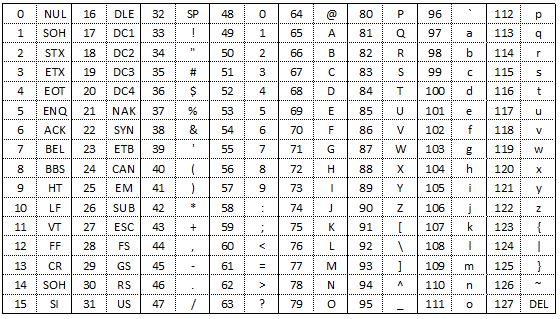
\includegraphics[width=0.24 \textwidth]{sections/ASCII-Tabelle}
\begin{tabular}{rlcrl}
	00-31:& NUL, ... & \quad & 32:& SPACE\\
	48-57:& 0-9& \quad &	65-90:& A-Z \\
	97-122:& a-z & \quad & 127:& DEL\\
\end{tabular}





	\section{Klassen}
Eine Klasse ist eine Datenstruktur wie auch Structs. Eine Klasse hat jedoch unterschiedliche Zugriffsrechte auf die internen Variabeln, Objekte genannt.
\begin{itemize}
	\item[\texttt{private}] - (default) Elemente, meist interne Variablen, können nur innerhalb der Klasse angesprochen werden. Memeberfunktionen(Methoden) können darauf zugreifen. 
	\item[\texttt{public}] - Elemente, die meisten Methoden, können von innerhalb und ausserhalb der Klasse angesprochen werden.
	\item[\texttt{protected}] - Elemente können von innerhalb der Klasse und von abgeleiteten Klassen angesprochen werden.
\end{itemize}
\begin{lstlisting}
	class klassenname{
		private:
			int n;					//Membervariabeln
			int d;
		public:
			Klassenname(int, int);	//Konstruktor
			int f1(int);			//Memeberfunktionen (prototyp)
			void f2();
	};
\end{lstlisting}
\subsection{Konstruktoren}
Konstruktoren sind spezielle Memeberfunktionen, die den Namen der Klasse tragen. Sie können auch überladen werden und werden bei der Variabelndeklaration aufgerufen.
\begin{lstlisting}
	class rational{
		...
		public:
		rational (int num, int den);
		rational ();
	};
	rational::rational (int num, int den)
	: n(num), d(den){ //Variabeln initialisierung
		assert(den!=0); // Funktionsrumpf
	}
	rational::rational () : n(0), d(1){};
\end{lstlisting}
Damit eine Variable bereits definiert werden kann ohne ''initialisiert'' zu werden, sollte ein Default-Konstruktor erstellt werden. Dieser enthält keine Argumente setzt die Membervariablen auf ein spezifischen default-Wert. Nun kann ein Objekt vom Typ rational unterschiedlich initialisiert werden. 
\begin{lstlisting}
	rational r
	rational r1(1,2);
	rational r2 = rational(1,2);
\end{lstlisting}
Der \texttt{this->}-Pointer ist ein Pointer auf das Aktuelle Objekt.




\end{multicols*}		

\end{document}
